\chapter{General Terms}\label{chap:general_terms}

\paragraph{Centroids}
Centroids are the centers of clusters.

\paragraph{Confidence Score} 
A score that tells you how accurate and reliable a model is performing based on the test data.

\paragraph{Convex}
%TODO bespreek convex hull, convex optimisation, in ieder geval da ding da we gebruiken voor de python tutorial 29 moeten we wel vermelden.

\paragraph{Cross Validation} 
Is a model validation technique for assessing how the results of a statistical analysis will generalize to an independent data set. It splits the data set in test and training data.

\paragraph{Deterministic Enviroment}
The endstate of the enviroment can be determined based on the current state of the enviroments and its components.

\paragraph{Decision Boundary}
In a statistical-classification problem with two classes, a decision boundary is a hyperplane that partitions the underlying vector space into two sets, one for each class.

\paragraph{Dot Product}
Also known as \emph{scalair product} or \emph{inner product} of two vectors $\vec{A}$ and $\vec{B}$ is defined as follows: $\vec{A} \cdot \vec{B} = a_1 b_1 + a_2 b_2 + ... + a_n b_n$. Two vectors are perpindicular if their dot product equals 0. Dutch translation: \emph{inwendig product}

\paragraph{Eucledian Distance}
A way to calculate the distance on a plane between points. It uses the following formula: $\sqrt{\sum\limits_{i=1}^n (q_{i} - p_{i})^2}$. Measures the length of a line segment between points.

\paragraph{Eucledian Norm}
Measures the magnitude of a vector, which is basically the length. The equation is also the same as with Eucledian Distance, the name just tells you what space you are using.

\paragraph{Features} 
Descriptive attributes for the data.

\paragraph{Hyperplane}
A hyperplane is a subspace of one dimension less than its ambient space. If a space is 3-dimensional then its hyperplanes are the 2-dimensional planes.

\paragraph{Kernels} 
Is a kind of transformation on your data. Grossly put it simplifies your data. More specifically kernel methods use kernel functions to operate in a high-dimensional, implicit feature space without ever computing the coordinates of the data in that space, but rather by simply computing the inner products between the images of all pairs of data in the feature space. This is computationally a lot better than using the raw data. For an example see figure \ref{fig:kernelmethods}.
\begin{figure}
\centering
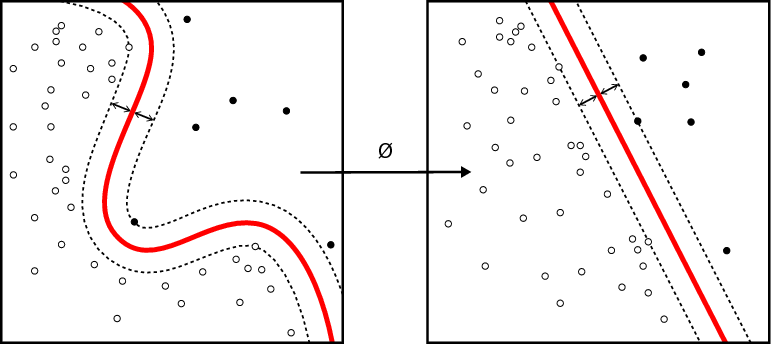
\includegraphics[width=0.4\textwidth]{images/kernelmethod.png}
\caption{\label{fig:kernelmethods} An example of simplifying the data by increasing it's dimension.}
\end{figure}

\paragraph{Labels} 
What you are trying to predict of forecast for the data.

\paragraph{Linear Algebra} 
The objective of linear algebra is to calculate relationships of points in vector space. 

\paragraph{(Maximum) Margin Classifier}
A margin classifier is a classifier which is able to give an associated distance from the decision boundary for each example. A maximum margin classifier maximises the distance between the decision boundary and all examples.

\paragraph{Object Oriented Programming}
In short OOP makes it possible to make objects with attributes, these objects can have a certain link towards eachother (subclasses and superclasses).
%TODO maak definitie OOP mooier

\paragraph{Preprocessing} 
Used to clean/scale the data before using machine learning techniques. Cleaning for example by replacing NaN data with -99 999, because it will be handled as an outlier, or by interpolating it. Scaling your features so they fall between -1 and 1 is genarally a good idea because it could make the processing faster and more accurate.

\paragraph{Machine Learning Classifier} %TODO

\paragraph{Machine Learning Model} %TODO

\paragraph{Norm} %TODO

\paragraph{Overfitting}
Figure \ref{fig:svm-overfitting} should explain overfitting perfectly.

\begin{figure}
\centering
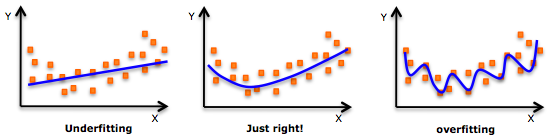
\includegraphics[width=0.8\textwidth]{images/svm-overfitting.png}
\caption{\label{fig:svm-overfitting} Shows underfitting, right fitting and overfitting.}
\end{figure}

\paragraph{Stochastic Enviroment}
The endstate of the enviroment can not be exactly determined based on the current state of the enviroment and its objects since there is randomness involved.

\paragraph{Supervised Learning} 
For om machine learning where the scientist teaches the machine by showing it features and then showing it the correct answer (lable). Once the machine is taught, the scientis will usually test the machine on some unseen data, where the scientis still knows the correct answer, but the machine doesn't.

\paragraph{R squared method}
Also known as \emph{coefficient of determination}. The squared error is the mean or sum of the distance between the solution values and the actual values. For example in Linear regression the error is the distance between the regresssion line's y values and the data's y values. The squared error is either a mean or sum of this. Squared error is used because on the one hand it normalises all errors to be positive and on the other hand it punishes outliers harder. Since the squared error is just a relative number to your dataset it has no real meaning, that's why we use the r squared method. This method uses the formula $r^2 = 1 - \frac{SE\hat{y}}{SE_{\overline{y}}}$ which is just one minus the division of the squared error of the regression line and the squared error of the mean y line. A number close to 1 means the classifier is performing well, a number close to 0 means it is performing bad. It is a good measure when trying to predict an exact future value, however if you just want to predict a general tendense it is not the best measure.

\paragraph{Support Vector}
The points closest to the maximum-margin-hyperplane, as shown in figure \ref{fig:svm-support-vectors}.

\paragraph{Threading} 
Some machine learning algorithms can be split into multiple threads, this is often indicated by the \emph{n\_ jobs} parameter in python. Others don't have this luxurary and are known as running linear.

\paragraph{Types of Data} 
With machine learning we can see our data in several groups. It is important that these groups do not overlap, since otherwise a bad representation of results could be shown.
\begin{itemize}
	\item \textbf{Training data} is the data used to train your machine learning model.
	\item \textbf{Testing data} is the data used to test your machine learning model.
	\item \textbf{Validation data} is the data used to validate your machine learning model.
\end{itemize}

\paragraph{Unsupervised Learning}
As opposed to supervised learning, the scientist doesn't tell the machine what the classes of featuresets were.

\paragraph{Vector}
A vector has a \emph{magnitude} and a \emph{direction}. The \emph{magnitude} is the same as the Euclidean distance or norm. For example the $\vec{A} = [4, 3]$ has the direction 4 in dimension 1 and 2 in dimension 2, the magnitudes is $\sqrt{4^2 + 3^2} = 5$. 


 
